\documentclass[tikz]{standalone}
\usepackage{tikz}
\usetikzlibrary{shapes.geometric}


% This bascially automates a \newcommand{<name>}{} to ensure
% that a command with the given <name> does not already exist
\newcommand*{\pgfmathsetnewmacro}[2]{%
    \newcommand*{#1}{}% Error if already defined
    \pgfmathsetmacro{#1}{#2}%
}%



\begin{document}


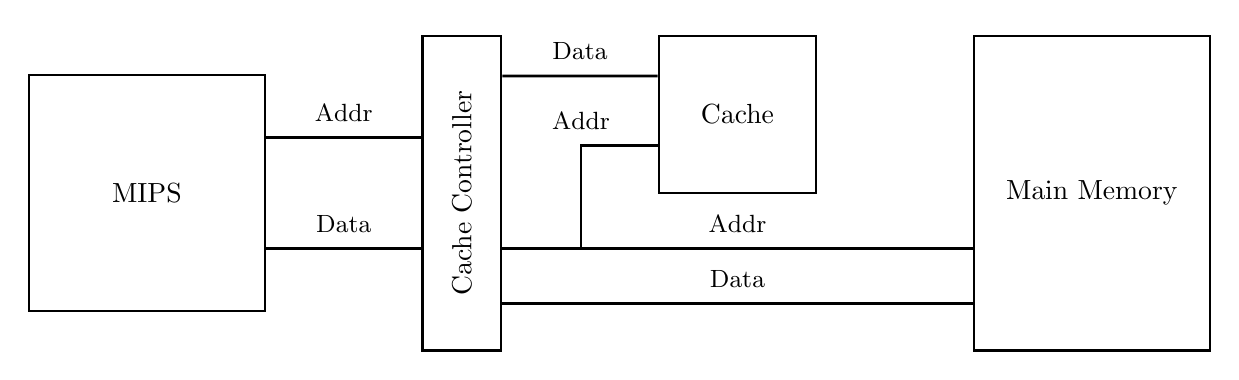
\begin{tikzpicture} 
	\tikzstyle{every node}=[draw, thick, minimum height=0.6cm, minimum width=1cm]

	// mips
	\node[minimum height=3cm, minimum width=3cm](MIPS) at (0, 0) {MIPS};

	// cache controller
	\node[minimum height=1cm, minimum width=4cm, rotate=90](Cache_Ctrl) at (4, 0) {Cache Controller};

	// cache
	\node[minimum height=2cm, minimum width=2cm](Cache) at (7.5, 1) {Cache};

	// memory
	\node[minimum height=4cm, minimum width=3cm](Memory) at (12, 0) {Main Memory};

	// lines
	// mips - cache controller
	// addr
	\draw[line width=1pt, font=\small]([yshift=20]MIPS.east)--([yshift=20]Cache_Ctrl.north) node[draw=none, anchor=south, midway]{Addr};
	// data
	\draw[line width=1pt, font=\small]([yshift=-20]MIPS.east)--([yshift=-20]Cache_Ctrl.north) node[draw=none, anchor=south, midway]{Data};
	
	// cache controller - memory
	// addr
	\draw[line width=1pt, font=\small]([yshift=-20]Cache_Ctrl.south)--([yshift=-20]Memory.west) node[draw=none, anchor=south, midway]{Addr};
	// data 
	\draw[line width=1pt, font=\small]([yshift=-40]Cache_Ctrl.south)--([yshift=-40]Memory.west) node[draw=none, anchor=south, midway]{Data};
	
	// cache controller - cache
	// data
	\draw[line width=1pt, font=\small]([yshift=-15]Cache_Ctrl.south east)--([yshift=-15]Cache.north west) node[draw=none, anchor=south, midway]{Data};
	// addr
	\draw[line width=1pt, font=\small]([yshift=-20]Cache_Ctrl.south)--++(1, 0)|-([yshift=-40]Cache.north west) node[draw=none, anchor=south, midway]{Addr};
	 
 
	


     
\end{tikzpicture}

\end{document}